\begin{frame}{Known Wilf classes}
    \begin{itemize}
        \item<1-> Classes avoiding one, two or three patterns of size $3$.
            \subitems{%
                \item All classes in \authcite{simionandschmidt}.
                \item The bijection we found for $\Av{123}$ and $\Av{132}$ seems to agree with theirs.
            }
        \item<2-> Classes avoiding one pattern of size $3$ and one of size $4$.
        \item<3-> $\Av{1234}$, $\Av{1243}$ and $\Av{1432}$.
        \subitems{%
            \item $\Av{2143}$ is missing.
        }
    \end{itemize}
\end{frame}
\begin{frame}{Known Wilf classes, $\Av{1234}$ and $\Av{1243}$}
    \begin{figure}
        \tikz{\draw [black, opacity=0] (0,0) rectangle (10,7.5);}
        \tikz [remember picture,overlay] \node at ([yshift=-.25cm,xshift=0cm]current page.center) {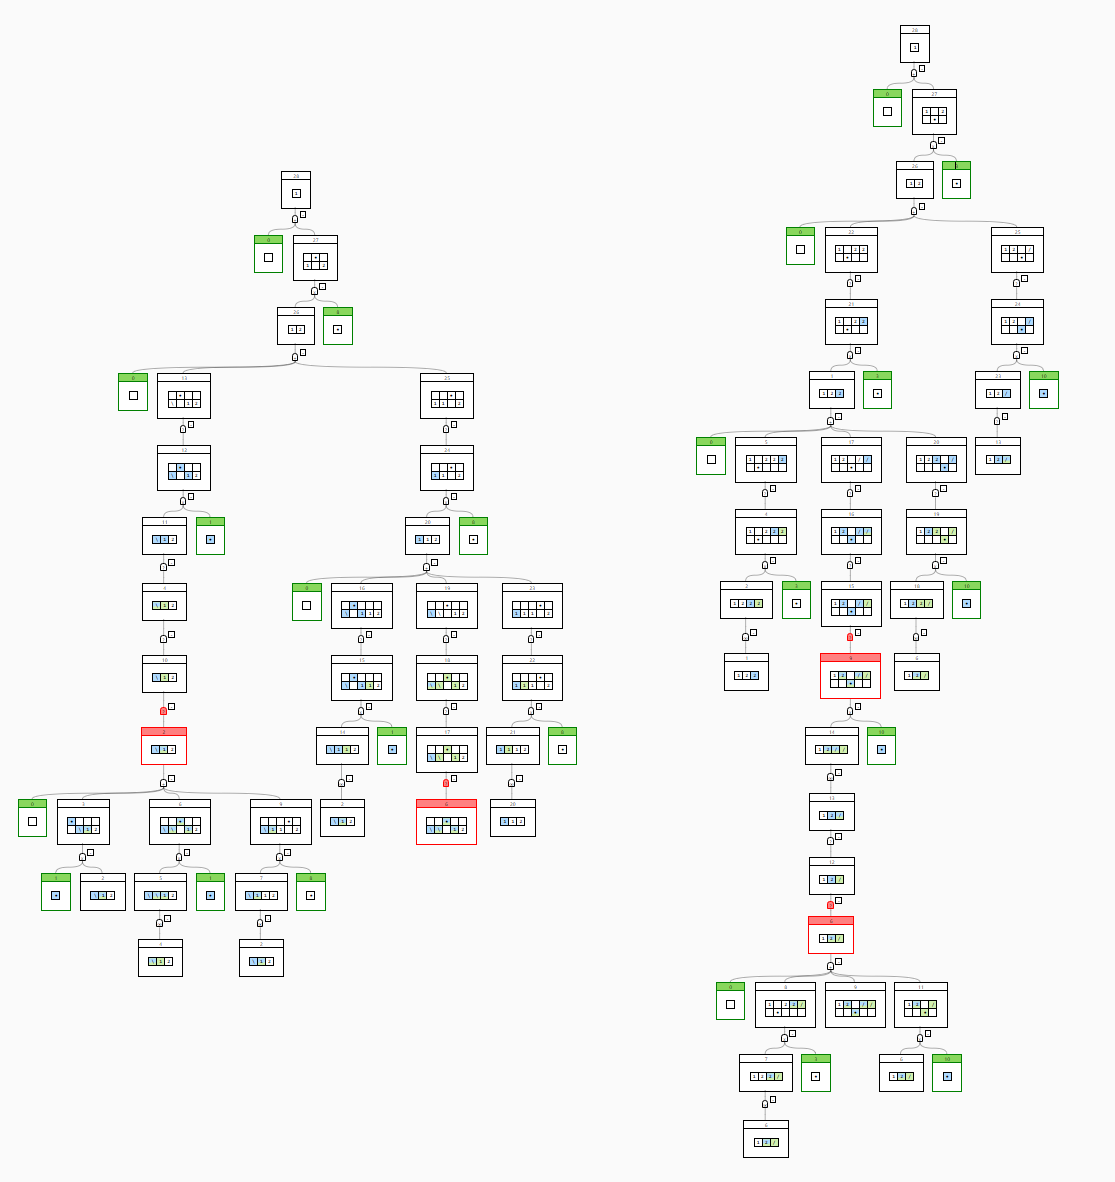
\includegraphics[scale=0.25]{graphics/1234_1243.png}};
        \caption{The parallel specifications found for $\Av{1234}$ and $\Av{1243}$.}
    \end{figure}
\end{frame}